% Section 3 - Simultaneous Localization And Mapping
% Roberto Masocco <roberto.masocco@uniroma2.it>
% June 5, 2024

% ### Simultaneous Localization And Mapping ###
\section{Simultaneous Localization And Mapping}
\graphicspath{{figs/section3/}}

% --- Simultaneous Localization And Mapping ---
\begin{frame}{Simultaneous Localization And Mapping}{Definition}
	The \textbg{SLAM} problem is a \textbg{chicken-and-egg} problem: a robot must \textbg{localize itself} within an environment, while \textbg{mapping} it.\\
	\bigskip
	The ultimate goal of SLAM is to enable the robot to \textbg{navigate} within the environment, while \textbg{updating} the map as it moves.\\
	\bigskip
	The robot must be able to \textbg{efficiently} and \textbg{accurately} build a map of the environment, while \textbg{localizing itself} within it, with respect to either the origin of the map or the starting point of the robot itself (\emph{i.e.}, with either some or none \textbg{prior notion of the environment}).\\
	\bigskip
	To solve this problem, \textbg{sensor fusion} techniques are often employed, mixing data coming from \textbg{heterogeneous sensors} and accounting for \textbg{sensor faults}.\\
  \bigskip
  Typically, SLAM algorithms rely on recognizable \textbg{features} of the environment to build the map and detect motion.
\end{frame}
\begin{frame}{Simultaneous Localization And Mapping}{Loop closure}
  \begin{columns}
    \column{.5\textwidth}
    While a SLAM system builds a \textbg{map} of the environment, it can detect whether it is exploring a zone that it has \textbg{already visited}.\\
    \medskip
    When this happens, the system can \textbg{close the loop} by \textbg{matching} the current "view" with a \textbg{previous one}, thus \textbg{correcting} the map and the robot's pose.\\
    \medskip
    This process is called \textbg{loop closure} and is a key feature of SLAM algorithms.\\
    \medskip
    Loop \textbg{detection} and \textbg{closing} must also be performed in real time, as well as the subsequent \textbg{corrections}; efficient optimization algorithms and data structures are crucial.

    \column{.5\textwidth}
    \begin{figure}
      \centering
      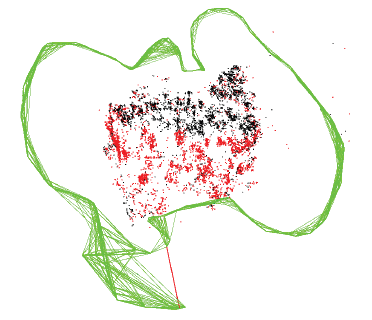
\includegraphics[width=.8\textwidth]{orbgraph}
      \caption{Loop closure of the ORB-SLAM2 algorithm.}
      \label{fig:loopclosure}
    \end{figure}
  \end{columns}
\end{frame}
\begin{frame}{Simultaneous Localization And Mapping}{Tools for the job}
  Sensors:
	\begin{itemize}
		\item \textbg{LIDARs} for direct environment mapping through depth information;
		\item \textbg{Cameras} to infer the environment structure through image processing;
		\item \textbg{IMUs} to account for the robot's motion and correct sampled data;
		\item \textbg{GNSS} to have a slow, but reliable global position estimate.
	\end{itemize}
  \medskip
  Plus all the \textbg{algorithms} and the \textbg{mathematical tools} we discussed in the context of \textbg{mapping}.
\end{frame}
\begin{frame}{Simultaneous Localization And Mapping}{Tools for the job}
  \begin{figure}
    \centering
    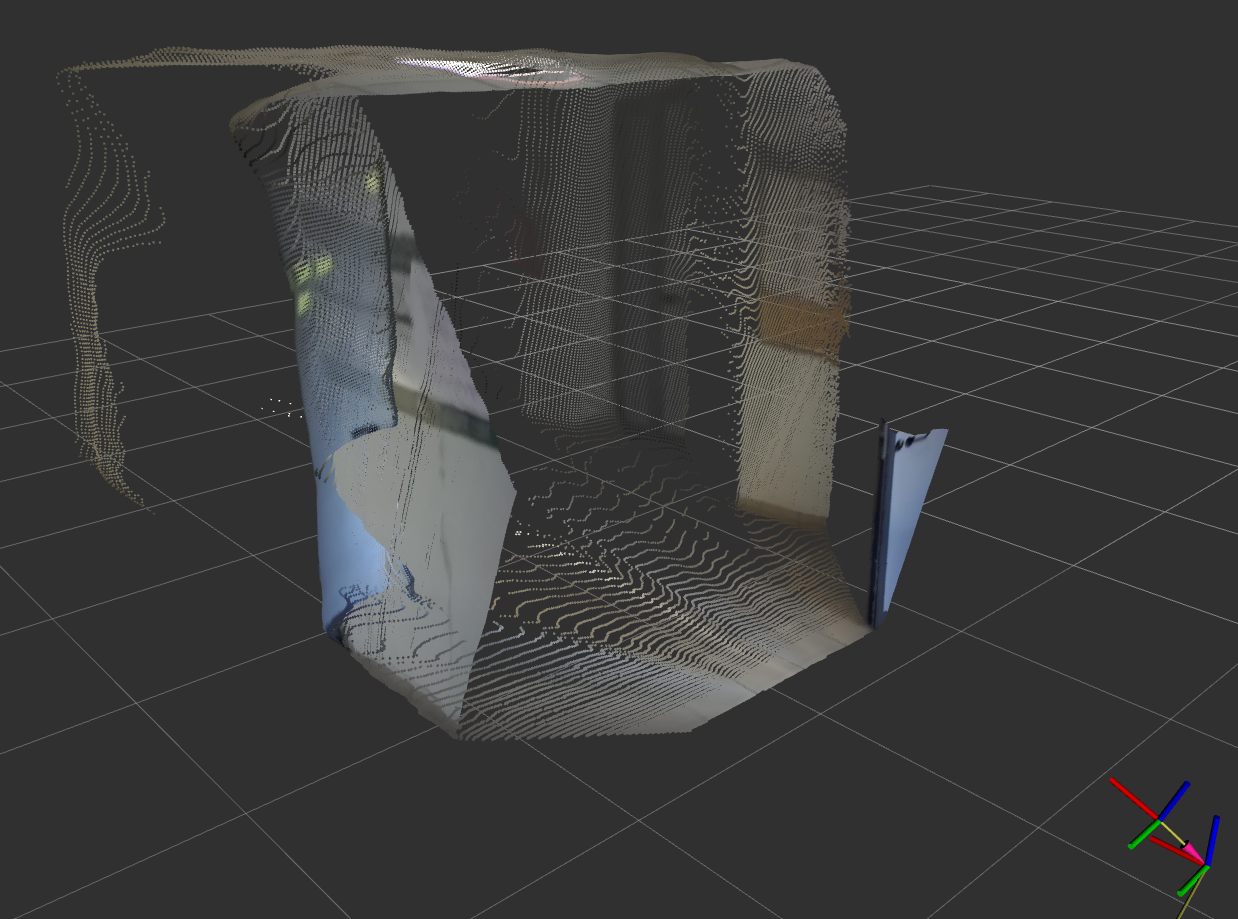
\includegraphics[width=.5\textwidth]{pointcloud}
    \caption{3D point cloud generated by a stereoscopic camera.}
    \label{fig:pointcloud}
  \end{figure}
\end{frame}

% --- 2D SLAM ---
\begin{frame}{2D SLAM}{Cartographer}
  \begin{columns}
    \column{.55\textwidth}
    \textbg{Cartographer} is a \textbg{2D} SLAM algorithm developed by Google.\\
    \medskip
    Meant for \textbg{offline} floor plan generation, it has been ported in \textbg{ROS} for mobile robot navigation.\\
    \medskip
    It used \textbg{LiDAR} laser scans, corrected by \textbg{IMU} data, to build 2D \textbg{submaps} of the \textbg{surrounding} environment.\\
    \medskip
    Such maps are then used to \textbg{build and update} a \textbg{global map}, gluing submaps together and optimizing the result.\\
    \medskip
    Features are particular \textbg{environment structures} that are used to detect loop closures and estimate the robot's trajectory.

    \column{.45\textwidth}
    \begin{figure}
      \centering
      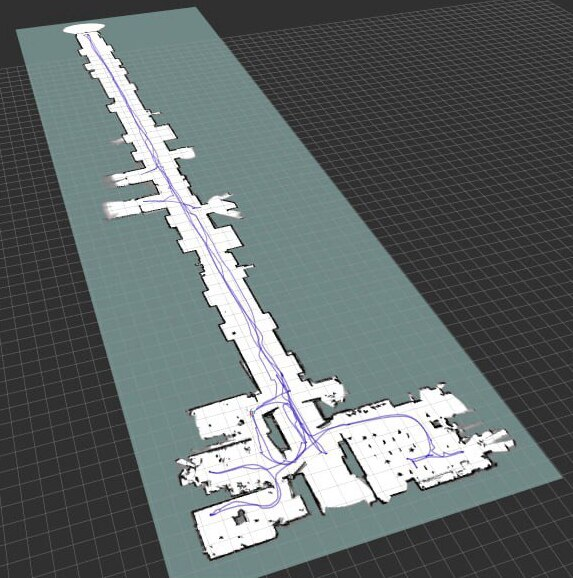
\includegraphics[width=.77\textwidth]{cartographer}
      \caption{Execution of the Cartographer SLAM algorithm.}
      \label{fig:cartographer}
    \end{figure}
  \end{columns}
\end{frame}

% --- Visual SLAM ---
\begin{frame}{Visual SLAM}{ORB-SLAM}
  \begin{columns}
    \column{.55\textwidth}
    \textbg{ORB-SLAM} is a \textbg{visual} SLAM algorithm that uses \textbg{monocular} or \textbg{stereo} cameras to build a map of the environment.\\
    \medskip
    It relies on \textbg{binary ORB features} to detect and match points in the environment, building a \textbg{covisibility graph} of \textbg{keyframes}: relevant views for pose estimation.\\
    \medskip
    The graph, and thus, the map and the camera pose estimate, are optimized with \textbg{bundle adjustment}.\\
    \medskip
    Latest versions also include \textbg{IMU} samples in the bundle adjustment cost function.

    \column{.45\textwidth}
		\begin{figure}
			\centering
			\movie[width=.85\textwidth, height=.6\textheight, poster, autostart, loop]{}{phd23_orb2-building-cut.mp4}
			\caption{ORB-SLAM2 algorithm execution on a ROS 2 dataset (bag).}
			\label{vid:building}
		\end{figure}
  \end{columns}
\end{frame}
